\documentclass[12pt]{amsart}
\usepackage{amsthm}
\usepackage{graphicx}
\newcommand*\oct{\vcenter{\hbox{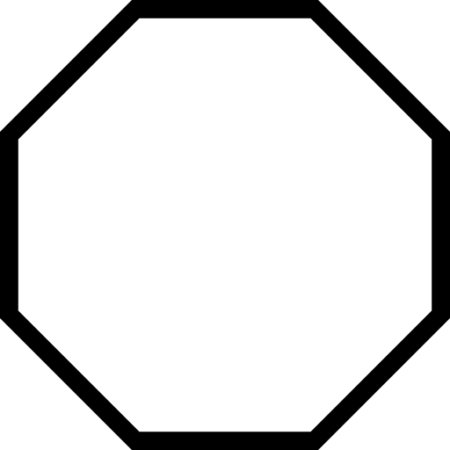
\includegraphics[width=.9em]{octagon.png}}}}
\newcommand{\F}{\mathcal{F}}
\newcommand{\Z}{\mathbb{Z}}

\newtheorem{theorem}{Theorem}
\newtheorem{lemma}{Lemma}
\newtheorem{corollary}{Corollary}

\theoremstyle{definition}
\newtheorem{definition}{Definition}

\title{Stopping Times}
\author{Robert Dougherty-Bliss and Charles Kenney}

\begin{document}
\maketitle

\begin{definition}
    A \emph{binary string of length $n$} is a tuple $(x_1, x_2, \dots, x_n)$
    where each $x_k$ is $0$ or $1$. Such a string is said to be \emph{stopped}
    at index $k$ if every index of the tuple in $(k / 2, k]$ is zero. The
    \emph{stopping time} of a binary string is the smallest $k$ such that the
    string is stopped at index $k$, or $\infty$ if no such $k$ exists. Note
    that, except $1$ and $\infty$, every stopping time is even.
\end{definition}

We are primarily interested in binary strings of length $n$ which have stopping
time $n$. Indeed, let $g(n)$ be the number of such strings. Our first goal is
to show that $g(n)$ satifies the recurrence
\begin{align*}
    g(1) &= g(2) = g(4) = 1 \\
    g(4n) &= 2 g(4n - 2) \\
    g(4n + 2) &= 2 g(4n) - g(2n).
\end{align*}
This will identify the sequence $a(n) = g(2n)$ as the
\emph{Narayana--Zidek--Capell numbers}, A2083 in the OEIS, which begin
\begin{equation*}
    1, 1, 1, 2, 3, 6, 11, 22, 42, 84, 165, 330, 654, \dots
\end{equation*}
This recurrence was discovered thanks to the OEIS.

Our first definition discusses \emph{finite} binary strings, but it is more
convenient to work with \emph{infinite} binary strings which are nonzero in
only finitely many places. This is equivalent, and has the benefit that every
such infinite string has a finite stopping time when considered as a
sufficiently long, finite binary string.

\begin{definition}
    Let
    \begin{equation*}
        V = \bigoplus_{k=1}^\infty (\Z/2\Z)
    \end{equation*}
    be the direct sum of infinitely many copies of $\Z / 2\Z$. That is, the set
    of all infinite tuples $(x_1, x_2, x_3, \dots)$ where each $x_k$ is $0$ or
    $1$, and only finitely many are $1$. For each positive integer $k$, let
    $\oct_k$ be the set of elements of $V$ which are zero beyond position $k$
    and, when the first $k$ entries are regarded as a finite binary string,
    they have stopping time $k$. That is, $\oct_1 = \{0\} \subset V$,
    \begin{equation*}
        \oct_{2k} = \{v \in V : \forall j > k, v_j = 0, \text{ and } v \text{ has stopping time } 2k \}
    \end{equation*}
    and $\oct_{2k + 1} = \emptyset$ for every integer $k \geq 1$.
\end{definition}

It is clear that $g(n) = |\oct_n|$ for every positive integer $n$.

\begin{theorem}
    The sequence $g(n)$ satisfies the recurrence
    \begin{align*}
        g(1) &= g(2) = g(4) = 1 \\
        g(4n) &= 2 g(4n - 2) \\
        g(4n + 2) &= 2 g(4n) - g(2n).
    \end{align*}
\end{theorem}

% Todo
% Clean this up!
% Add details!
% (I [Robert] volunteer to do this.)
\begin{proof}
    Each nonzero element in $V$ has a final nonzero entry. Let $e_0 \colon V
    \to V$ be a map which inserts a $0$ in the position of this final entry,
    shifting the previous entry to the right. Similarly, let $e_1$ insert a $1$
    into this position. Symbolically,
    \begin{equation*}
        e_0(b) =
            \begin{cases}
                0 \text{ if } b=0 \\
                (b_1, ..., b_j, 0, 1, 0,0,...) \text{ if } b = (b_1, ..., b_j, 1, 0, 0, ...)
            \end{cases}
    \end{equation*}
    and
    \begin{equation*}
        e_1(b) =
            \begin{cases}
                (1, 0, 0, \dots) \text{ if } b=0 \\
                (b_1, ..., b_j, 1, 1, 0,0,...) \text{ if } b = (b_1, ..., b_j, 1, 0, 0, ...)
            \end{cases}.
    \end{equation*}
    Note that $e_0$ and $e_1$ are injective, $e_0(V) \cap e_1(V) = \emptyset,$
    and $e_0(V) \cup e_1(V) = V.$

    For any positive integer $k$,
    \begin{equation*}
        \oct_{2k + 2} \subseteq e_0(\oct_{2k}) \cup e_1(\oct_{2k}).
    \end{equation*}
    Indeed, the final nonzero entry of every string in $\oct_{2k + 2}$ occurs
    at position $2k + 1$. Removing the immediately preceding entry produces a
    string in $\oct_{2k}$---$e_0$ and $e_1$ simply add the entry back.

    In the other direction, for $k \geq 2$ we have
    \begin{equation*}
        e_1(\oct_{2k}) \subseteq \oct_{2k + 2},
    \end{equation*}
    because inserting a $1$ into position $k$ will never decrease the stopping
    time. For \emph{odd} $k \geq 2$ we have
    \begin{equation*}
        e_0(\oct_{2k}) \subseteq \oct_{2k + 2},
    \end{equation*}
    because inserting a $0$ at position $k$ will only decrease the stopping
    time if the new stopping time \emph{is} $k$; this is impossible if $k$ is
    odd. This shows that
    \begin{equation*}
        S_{2k + 2} = e_0(S_{2k}) \cup e_1(S_{2k}),
    \end{equation*}
    and thus
    \begin{equation*}
        g(2k + 2) = 2 g(2k)
    \end{equation*}
    for $k$ odd.

    To handle the even case, let
    \begin{equation*}
        \oct_{2k}^1 = \{(b_1, ..., b_{2k}, 1, 0,0,...) \in V \text{ s.t. } (b_1,...,b_{2k},0,0,...) \in \oct_{2k}\}.
    \end{equation*}
    (Note that $|\oct_{2k}^1| = |\oct_{2k}| = g(2k)$.) Then
    \begin{equation*}
        e_0(\oct_{4k}) \subseteq \oct_{4k + 2} \cup \oct_{2k}^1.
    \end{equation*}
    This implies
    \begin{equation*}
        \oct_{4k + 2} \cup \oct_{2k}^1 = e_0(\oct_{4k}) \cup e_1(\oct_{4k}).
    \end{equation*}
    (That the left contains the right is clear given the preceding inclusion.
    For the other direction, the only problem is $\oct_{2k}^1 \subseteq
    e_0(\oct_{4k}) \cup e_1(\oct_{4k})$. This is easily handled by considering
    the element immediately preceding the final nonzero element.) Therefore
    \begin{equation*}
        g(4k + 2) + |\oct_{2k}^1| = 2 g(4k),
    \end{equation*}
    or
    \begin{equation*}
        g(4k + 2) = 2 g(4k) - g(2k).
    \end{equation*}
    This establishes the recurrence.
\end{proof}

\end{document}
